\documentclass[beamer]{standalone}

\usepackage{tikz}

\usetikzlibrary{backgrounds}
\usetikzlibrary{calc}
\usetikzlibrary{positioning}

\definecolor{x-red}{HTML}{e41a1c}
\definecolor{x-blue}{HTML}{3694E0}
\definecolor{x-green}{HTML}{63E05F}
\definecolor{x-purple}{HTML}{D365E3}
\definecolor{x-orange}{HTML}{E8A100}
\definecolor{x-yellow}{HTML}{fff200}

\definecolor{almost-white}{HTML}{f0f0f0}


\begin{document}

\begin{standaloneframe}

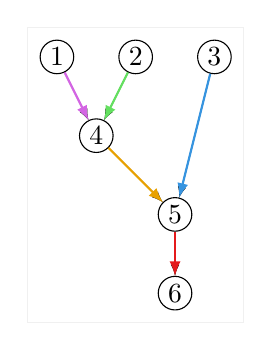
\begin{tikzpicture}[
    node/.style={draw, circle,
        inner sep=.05cm,
    },
    wire/.style={-latex},
    background rectangle/.style={ draw=almost-white, line width=0pt, },
    show background rectangle,
]

% other graph
\node [node] (n1) at (0,3) {\(1\)};
\node [node] (n2) at (1,3) {\(2\)};
\node [node] (n3) at (2,3) {\(3\)};
\node [node] (n4) at (.5,2) {\(4\)};
\node [node] (n5) at (1.5,1) {\(5\)};
\node [node] (n6) at (1.5,0) {\(6\)};

\onslide<1>{
    \draw [wire] (n1) to (n4);
    \draw [wire] (n2) to (n4);
    \draw [wire] (n4) to (n5);
    \draw [wire] (n3) to (n5);
    \draw [wire] (n5) to (n6);
}

\onslide<2>{
    \draw [wire, x-purple, thick] (n1) to (n4);
    \draw [wire, x-green, thick] (n2) to (n4);
    \draw [wire, x-orange, thick] (n4) to (n5);
    \draw [wire, x-blue, thick] (n3) to (n5);
    \draw [wire, x-red, thick] (n5) to (n6);
}

\end{tikzpicture}


\end{standaloneframe}

\end{document}
